\chapter{Design and Implementation of the Image Sequence Processing System for Motion Analysis}\label{chap:system_implementation}

In this chapter, I will show the different steps in the process of developing the software system designed to estimate vehicle motion.

\section{Sequencer as a way to step through the footage}
First, we need a way to step through the footage of the race car efficiently. In a finished product there is of course only one way to step through the footage: frame after frame. However, as we want to experiment with different frames, we need to be able to go through the footage quickly and easily.\bigskip

For this purpose, a sequencer is built, this sequencer takes footage from a camera mounted to a racing car. The footage from the camera is a video, to process this, each frame of the video is stored as a separate image. These images can be fed to the sequencer to process them. The sequencer takes 1 of these images at a time as input and stores it in a buffer. This image is converted into a grayscale image and cropped so the horizon is (as much as possible) out of the image. This converted image is then inserted into a FIFO of length N (right now, N is set at two). The two images in the FIFO are now ready for processing, the specifics of this processing will be discussed later. The visualisation component takes the images in the FIFO to visualise everything (keypoints, motion vectors...).\bigskip

With specific keys, it is possible to go forwards and backwards through the sequence. When advancing through the sequence a new image is loaded in the buffer. It is also possible to jump multiple frames ahead/backwards. The buffer is then cleared and filled with the correct images. With a press of the space bar, the sequencer continuously takes the next input image and loops the sequence.\bigskip

Figure \autoref{fig:scheme} shows an overview of the different steps the sequencer goes through. The "Process Image Pair" component calculates the Homography $\MH$ between the two frames in the FIFO. Based on the Homography, the rotation matrix $\MR$, translation vector $\vt$ and normal vector $\vn$ can be calculated which will be used to estimate the motion of the car.

\begin{figure}
    \centering
    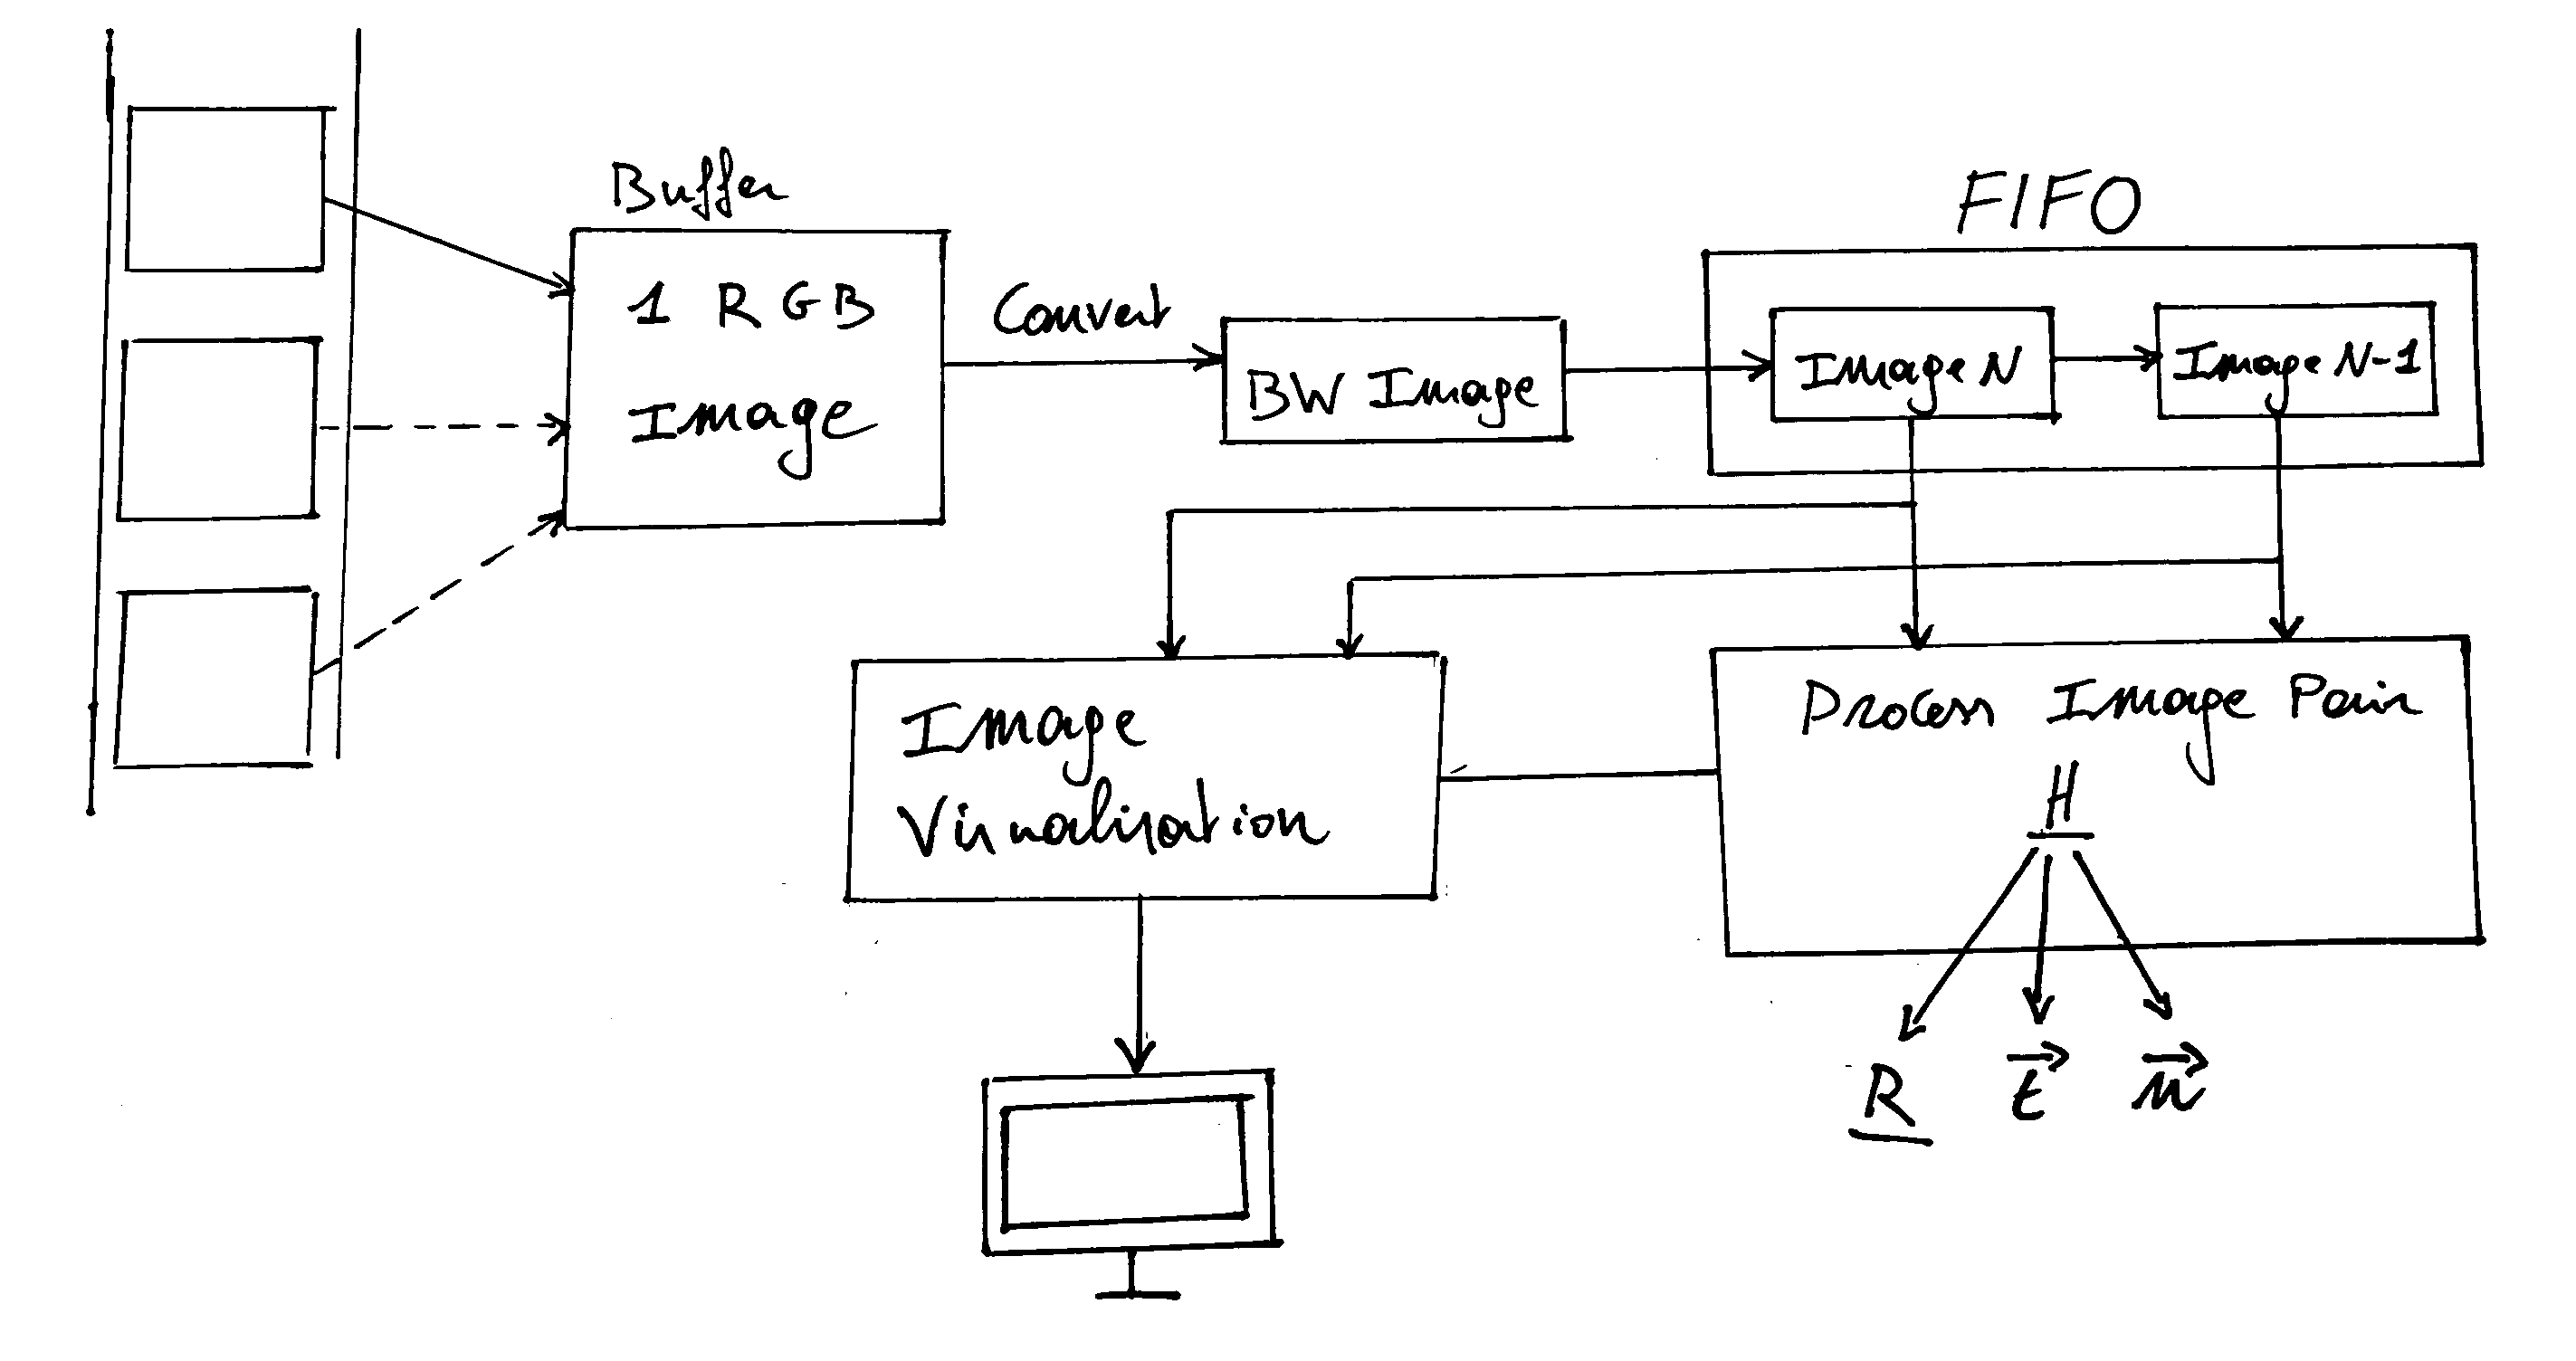
\includegraphics[width=1\textwidth]{figures/Block_diagram_sequencer.jpg}
    \caption{Scheme of sequencer}
    \label{fig:scheme}
\end{figure}

\section{Converting input image}
\subsection{Grayscale or color}
For now, the images are converted to grayscale. The big advantage is that a grayscale image only has one third of the information of an image in color with the same dimensions. Computationally everything will be faster using grayscale instead of color images. The drawback is a loss of information, but that drawback is rather small. The color of the image does not give us much more information to recognise structure and detect keypoints. So it is not worth the extra computations.\bigskip

However, in the footage we are using, the road is marked by colored cones. Most of the time the road is marked by yellow cones but sometimes there are blue cones on the road which means the car should slalom in between these cones. If at one point it should turn out the color of the cones is necessary, this will not be a problem. The newest image is always stored in the buffer in its original color, if we want to determine the color of the cone, this can easily be done by looking at the area where the cone is located on the original image.

\subsection{Removing irrelevant information}\label{ssec:irrelevant}
As said before, the images are converted to grayscale. Next to that, they are also cropped. For now, we are only interested in what is going on below the horizon, as we focus on the homography we only need the road surface. In the footage we are using, there is not much to be cropped, because the footage we have is from a camera that was mounted tilted. Now that the sky and everything above the horizon is cropped out, there is one part of converting left.

\subsection{Masking out the ego-car}
\label{ssec:egocar}
The car itself is not moving relative to the camera, as the camera is fixed to the car, so it is irrelevant for the estimation of the movement. A mask is created to erase the car from the footage. This is only done when displaying the image however, otherwise the computation of keypoints would not work properly. When detecting the keypoints in the next step, keypoints laying in the area masked out by the ego-car, can be removed as keypoints. This is done by giving the mask as a parameter to OpenCV when computing the keypoints. Figure \autoref{fig:input_image} shows an example of a frame before it is preprocessed. Figure \autoref{fig:output_image} shows the image after preprocessing. The black part is the masked out ego-car.

\begin{figure}
    \centering
    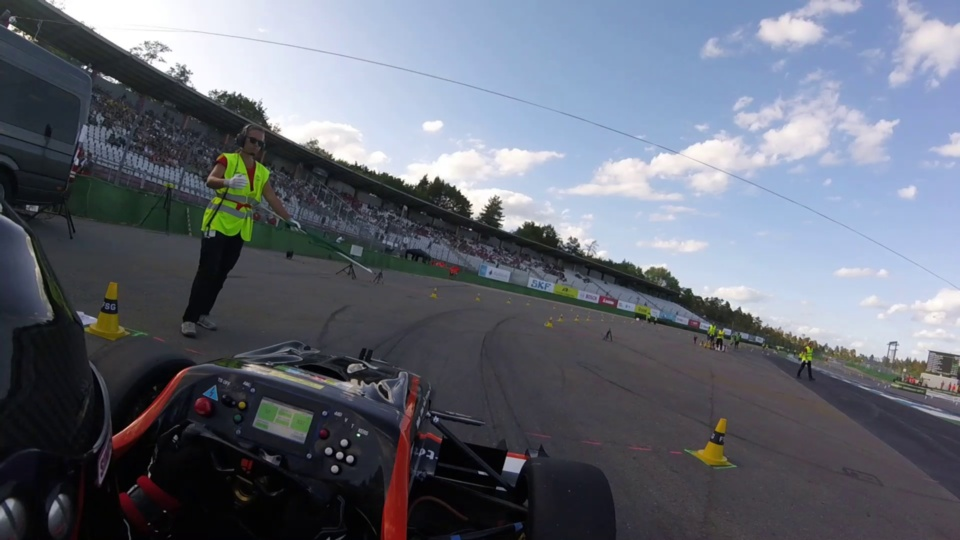
\includegraphics[width=1\textwidth]{figures/input_image.jpg}
    \caption{Input image}
    \label{fig:input_image}
\end{figure}

\begin{figure}
    \centering
    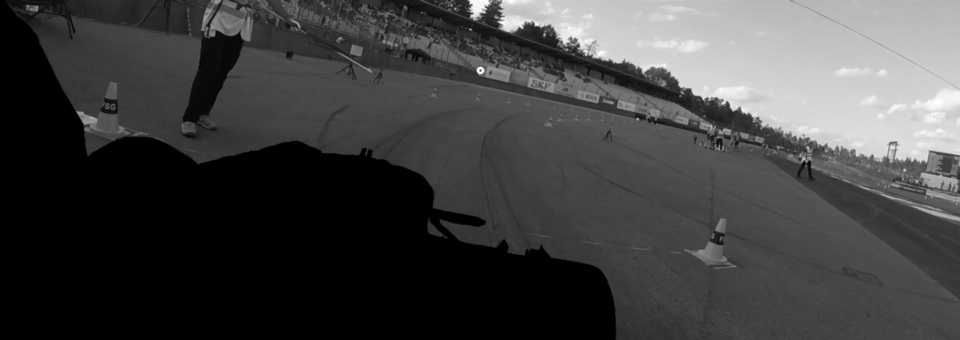
\includegraphics[width=1\textwidth]{figures/output_image.jpg}
    \caption{Preprocessed image}
    \label{fig:output_image}
\end{figure}

\section{Frame-to-frame 2D motion analysis}
We can now step through the footage efficiently. To estimate the frame-to-frame motion of the car, the rotation matrix $\MR$, translation vector $\vt$ and normal vector $\vn$ must be calculated. These can be calculated using keypoints in the frames. 

\subsection{Finding keypoints}
When the next image is loaded into the FIFO, we can detect the keypoints. As discussed in \autoref{sec:orb}, we use ORB. To find the keypoints we use the method \textit{detectAndCompute} on this image. We set the maximum amount of keypoints to a high 8000 for now. As we'll be using only a part of these, it isn't the best strategy computation wise. However, this ensures that we have enough keypoints as the road surface does not always have a lot of texture. \bigskip

\begin{figure}
    \centering
    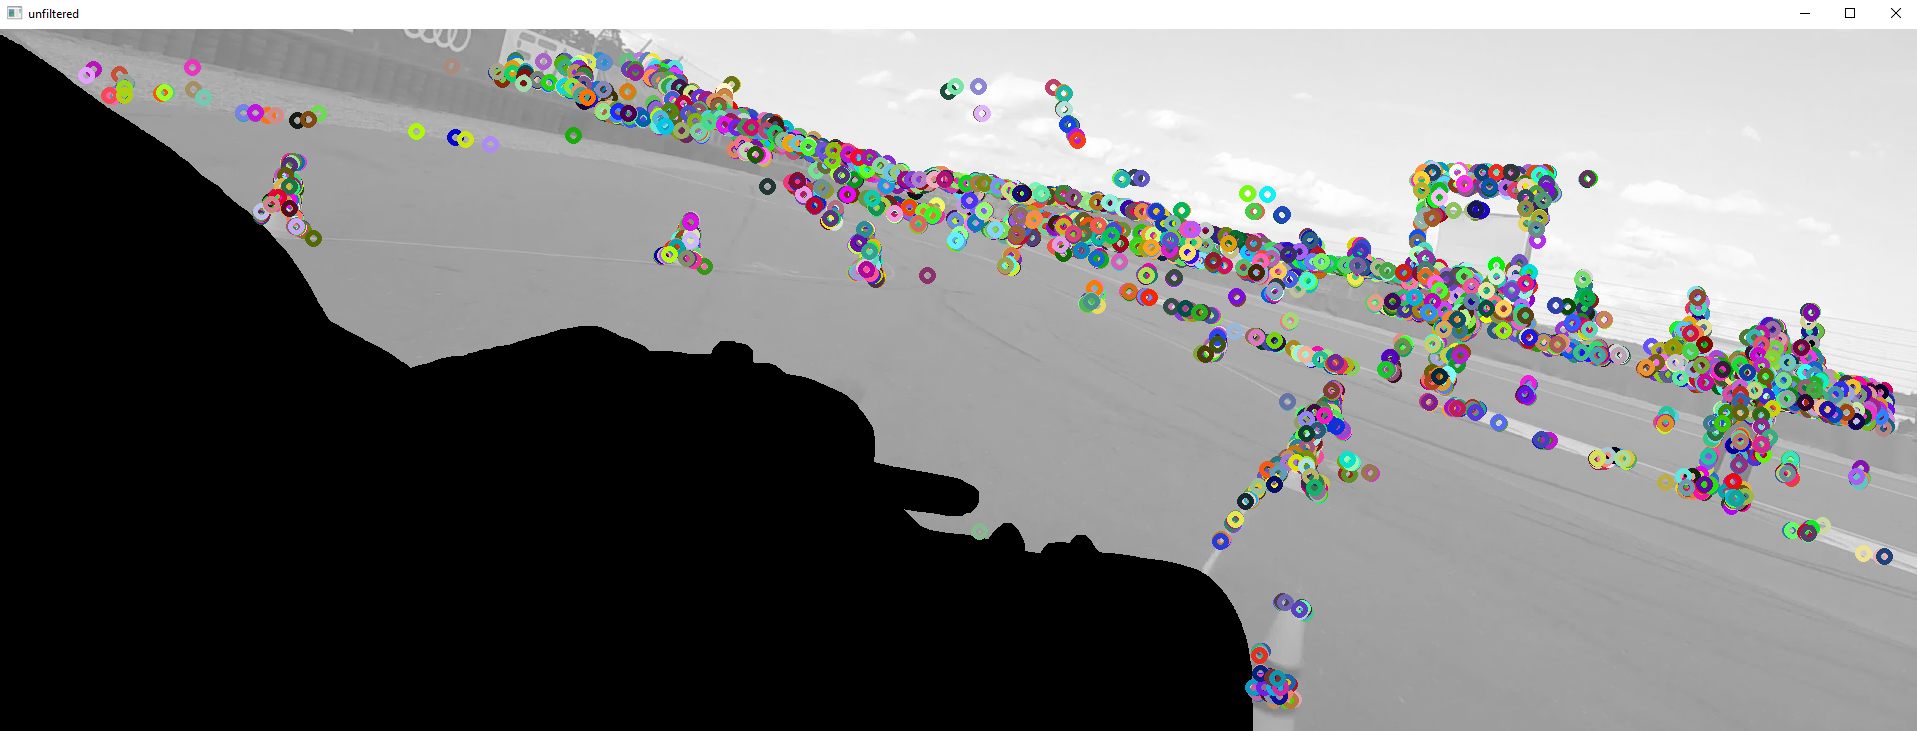
\includegraphics[width=1\textwidth]{figures/Unfiltered_keypoints.png}
    \caption{Detected keypoints before filtering}
    \label{fig:unfiltered}
\end{figure}

\subsection{Filtering keypoints}\label{ssec:filtering}

\autoref{fig:unfiltered} shows a frame with it's detected keypoints. Two things are clear: we have an excess of keypoints and they come in certain clusters. Thus we need to remove a big chunk of these keypoints, while trying to ensure we have a keypoint from the different clusters. To do this we work with a bucketing system. This means the image is divided into buckets. A bucket is a patch of the image, patches have no overlap and all patches together form the image.\bigskip 

The reason we have to use this bucketing system and remove the overall clustering of the keypoints can be found in \cite{6153423}. Fraundorfer and Scaramuzza state that "the keypoints should cover the image as evenly as possible".\bigskip 


Practically we divided the image in a grid of 40 by 20, leaving us with 800 buckets. Each of these buckets will have a maximum of 1 keypoint at the end, of course if there was no keypoint present in a bucket before filtering, there will not be a keypoint after filtering. \autoref{fig:bucketing} shows the result after filtering out the keypoints using the bucketing system.\bigskip

\begin{figure}
    \centering
    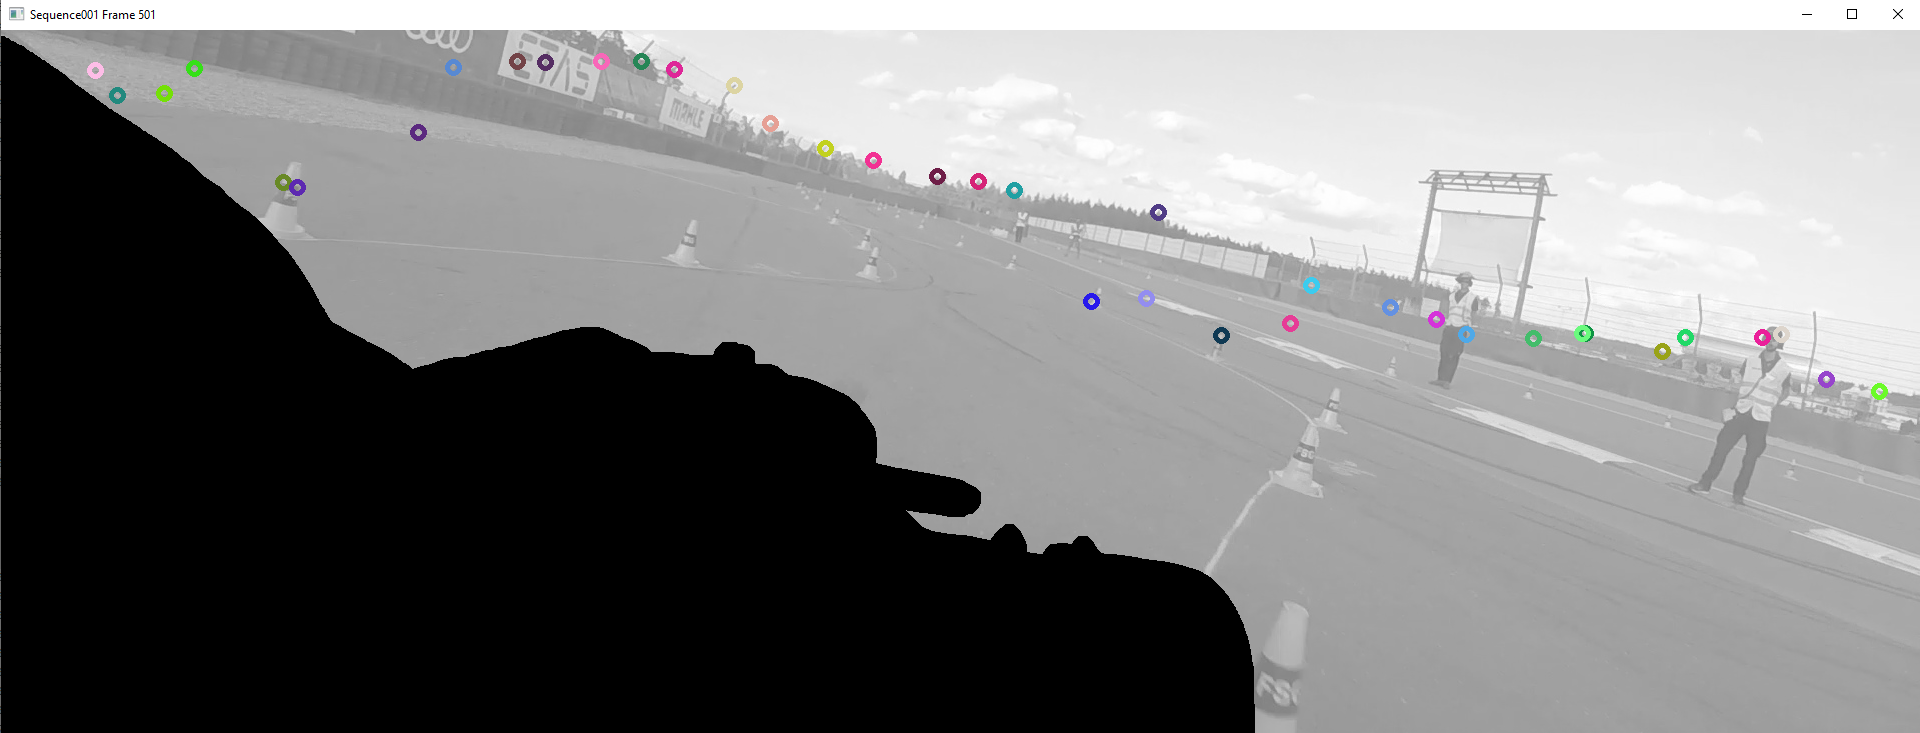
\includegraphics[width=1\textwidth]{figures/bucketing_filtered.png}
    \caption{Detected keypoints after bucketing}
    \label{fig:bucketing}
\end{figure}

As discussed before, we are looking for keypoints that are part of the road surface. Keypoints above the horizon can thus be discarded as we can say with absolute certainty that these will not be a part of the road surface. For now, we will determine the horizon empirically, in a later stage, when we have found the normal vector $\vn$ it will be possible to estimate the horizon based on this.\bigskip

As stated before, the footage we have is from a camera that is mounted tilted. This means we are not able to simply discard all keypoints above a horizontal line. We describe the horizon as a linear equation of the form
\begin{equation}\label{eq:linear}
    ax + by + c = 0
\end{equation}
To find the values for $a$, $b$ and $c$ we need two points on the horizon $p_1 = (x_1, y_1)$ and $ p_2 = (x_2, y_2)$. The slope of the line is then defined as $\frac{y_2-y_1}{x_2-x_1}$ if $x_1 \neq x_2$. A non-vertical line can be defined by its slope $m$, which we just defined and coordinates of any point on the line \cite{wiki_linear}:
\begin{equation}\label{eq:slope}
    y - y_1 = m(x-x_1)
\end{equation}
\autoref{eq:slope} can then be rewritten in terms of $p_1$ and $p_2$ as follows:
\begin{equation}
    y - y_1 = \frac{y_2-y_1}{x_2-x_1}(x-x_1)
\end{equation}
Multiplying both sides by $(x_2-x_1)$ gives the following equation, which is also valid when $x_1 = x_2$:
\begin{equation}
    (x_2-x_1)(y-y_1) - (y_2-y_1)(x-x_1) = 0
\end{equation}
which can be rewritten as
\begin{equation}
    (y_1-y_2)x + (x_2-x_1)y + (x_1y_2-x_2y_1) = 0
\end{equation}
For now an estimation suffices so we chose two points empirically. In \autoref{ssec:irrelevant} we already chose a height to cut off irrelevant information, this height was chosen based on the horizon. For $p_1$ we take this height as $y_1$ and as the camera is tilted to the right this is the leftmost point and $x_1 = 0$. For $p_2$ we chose a point at the utmost right of the image so $x_2$ is equal to the width of the image. For $y_2$ we choose a value by simply looking what seems to be the best option. \bigskip

\autoref{fig:horizon} shows the same original image after filtering away the points that lay above the horizon. For illustration purposes, the horizon is drawn. Finally, in \autoref{fig:filtered} shows the keypoints that are left over after filtering, these are the keypoints we will work with.\bigskip

\begin{figure}
    \centering
    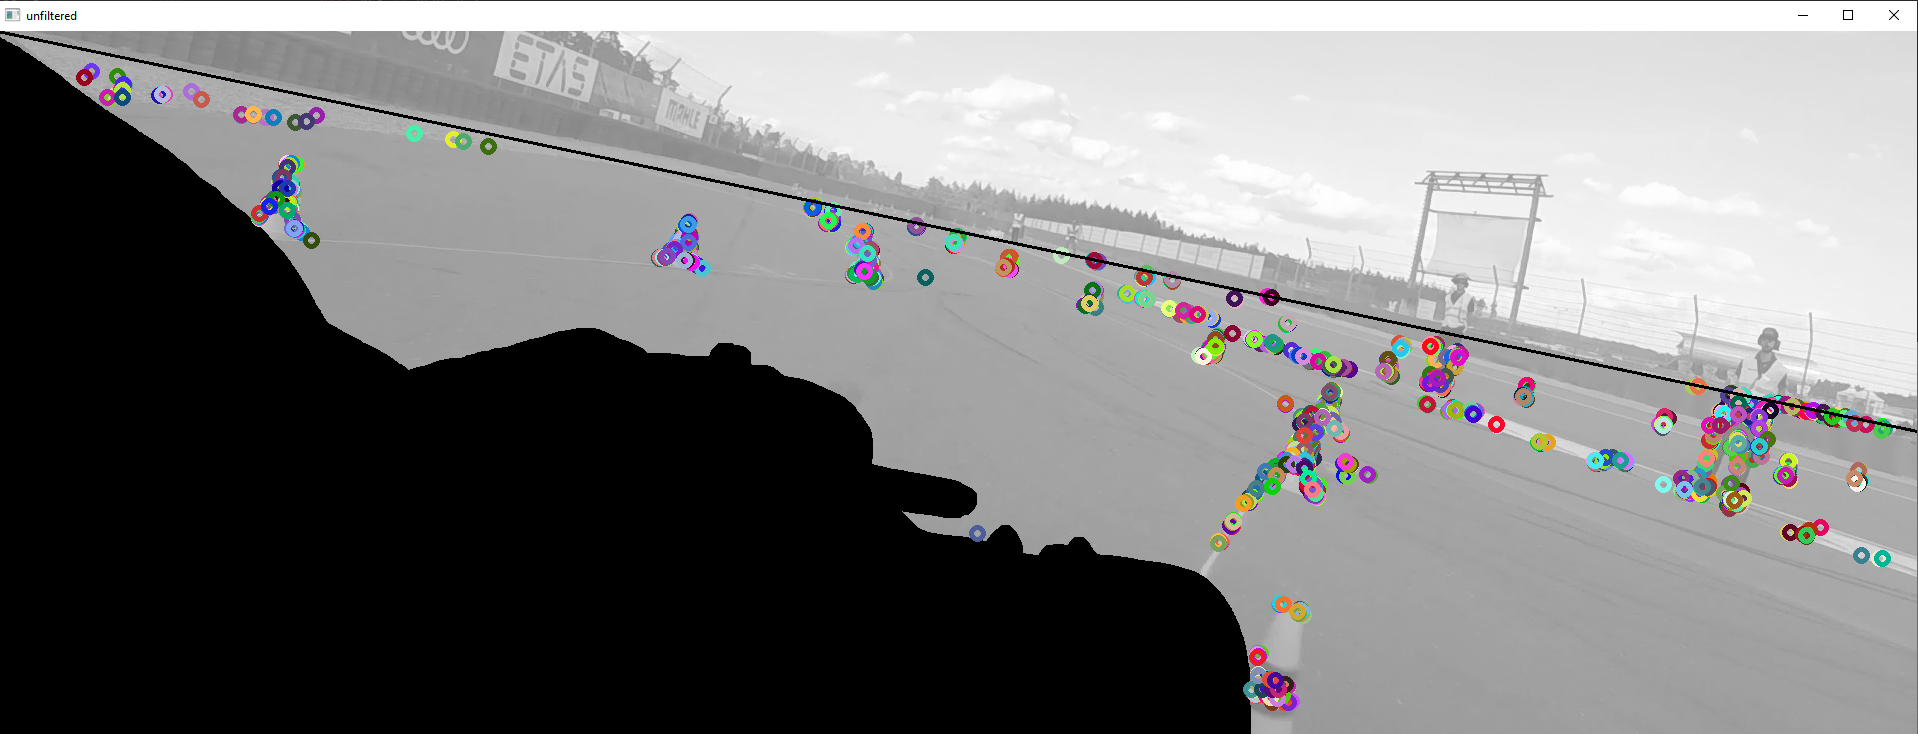
\includegraphics[width=1\textwidth]{figures/Horizon_filtered.png}
    \caption{Detected keypoints after removing keypoints above the horizon}
    \label{fig:horizon}
\end{figure}
\begin{figure}
    \centering
    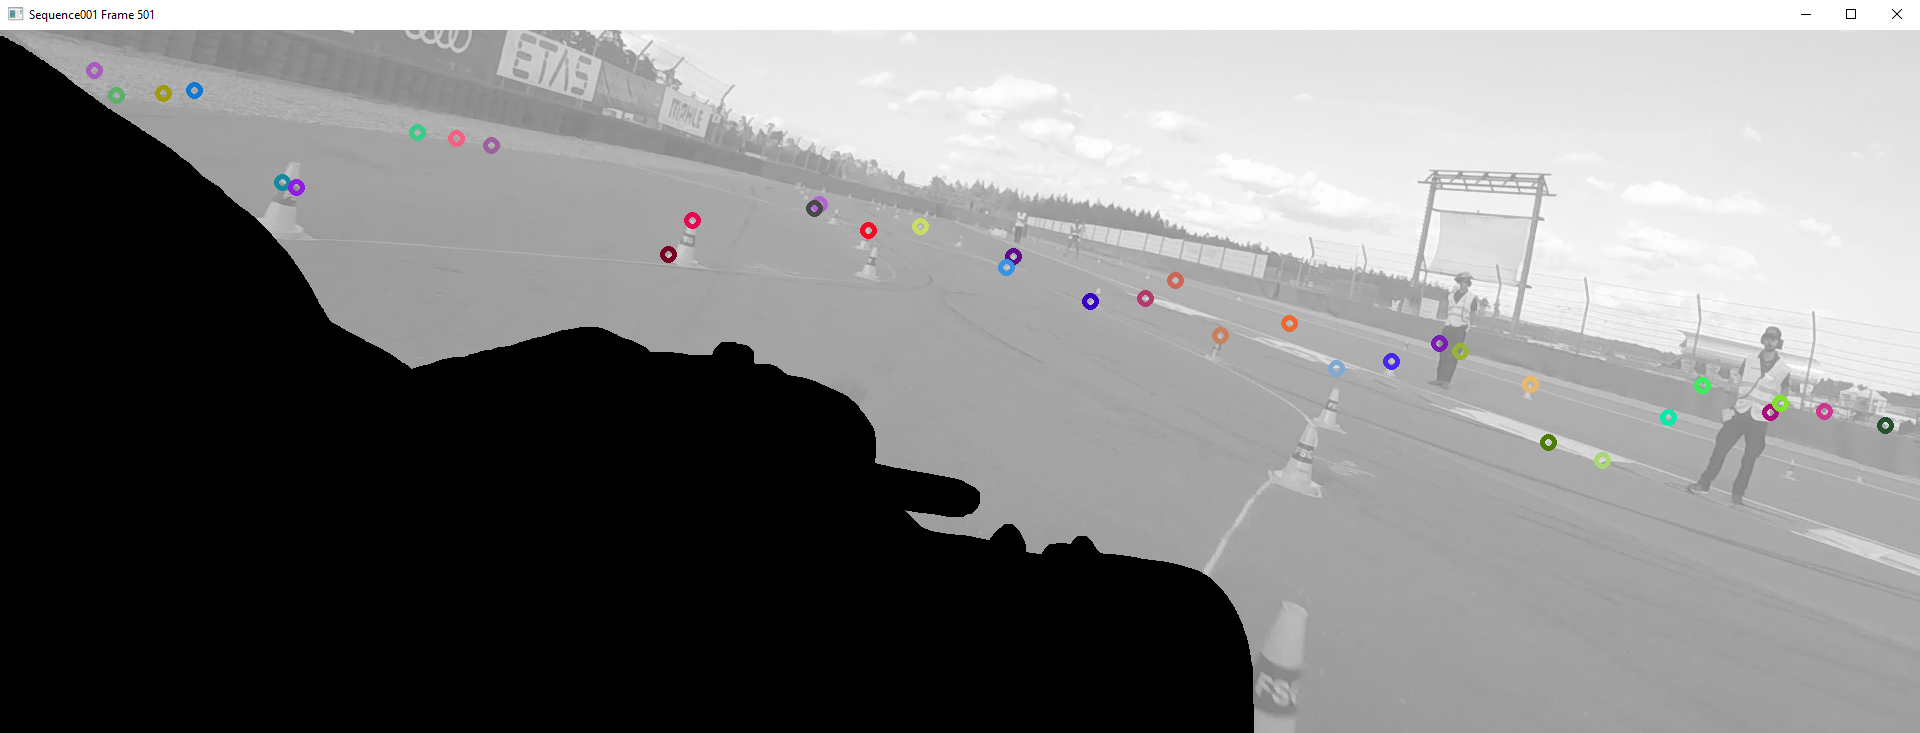
\includegraphics[width=1\textwidth]{figures/Filtered_keypoints.png}
    \caption{Detected keypoints after bucketing and removing keypoints above the horizon}
    \label{fig:filtered}
\end{figure}

For illustrating purposes, the contrast in the images is lowered by mapping the gray values between [0, 255] to [128, 255]. By doing this, the image is still clearly visible to the human eye but keypoints and the motion vectors are more visible.

\subsection{Matching keypoints}
The point in finding the keypoints is to know where these specific points are in another image. Note that the filtering described in \autoref{ssec:filtering} is only done on the oldest image. If we were to filter both images, chances are big we would be left with no good matches. After all, there is no way of guaranteeing that the right match of a keypoint that is not filtered will also be unfiltered in the second image.\bigskip

We use a brute force Hamming descriptor matcher, this means matches are made based on the Hamming distance between descriptors. Brute force means that every possible match is made for a certain keypoint after which the best match for that specific keypoint is chosen. The OpenCV \textit{match} method returns a list of matches based on this principle.\bigskip

When we look at the matches, draw both keypoints and connect them, what we should see is a bunch of motion vectors. However, looking at \autoref{fig:matches}, this is clearly not the case. Not all the matches we got are good matches, so once again we have to filter out the good ones.\bigskip

\begin{figure}
    \centering
    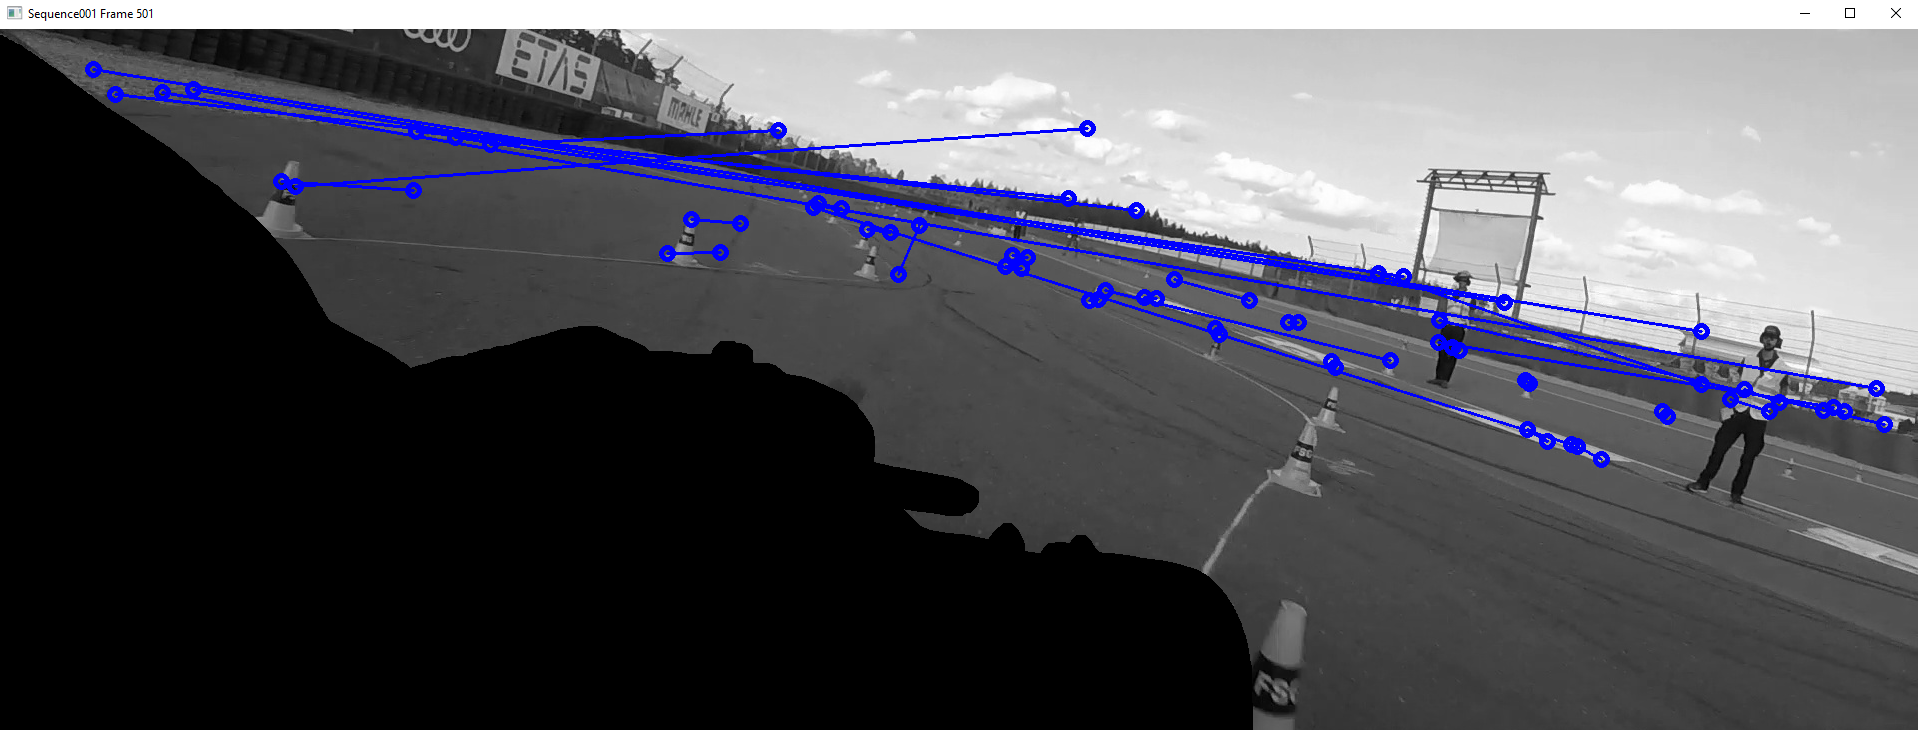
\includegraphics[width=1\textwidth]{figures/keypoint_matches.png}
    \caption{Keypoint matches}
    \label{fig:matches}
\end{figure}

The algorithm to calculate the homography is very prone to even the smallest outliers and mistakes. To prevent this, we look at the estimated matches one by one to look if it is actually a good match. We look at patches from around both keypoints while also factoring in the motion vector. \autoref{fig:match_check} shows a screenshot of this process. This is clearly a good match, the two patches are very similar and the motion vector drawn is plausible in this scenario. \autoref{fig:bad_match} however shows a match that is clearly a mistake, this match will not be considered anymore.\bigskip

Recall that we are looking for a homography between the ground plane in the two frames. So we can only use keypoints that are on the road surface. While checking if the keypoints are correctly matched, we also check if this is the case. After checking all this, we are left with good matches between keypoints in the two frames, that are part of the road surface.

\begin{figure}
    \centering
    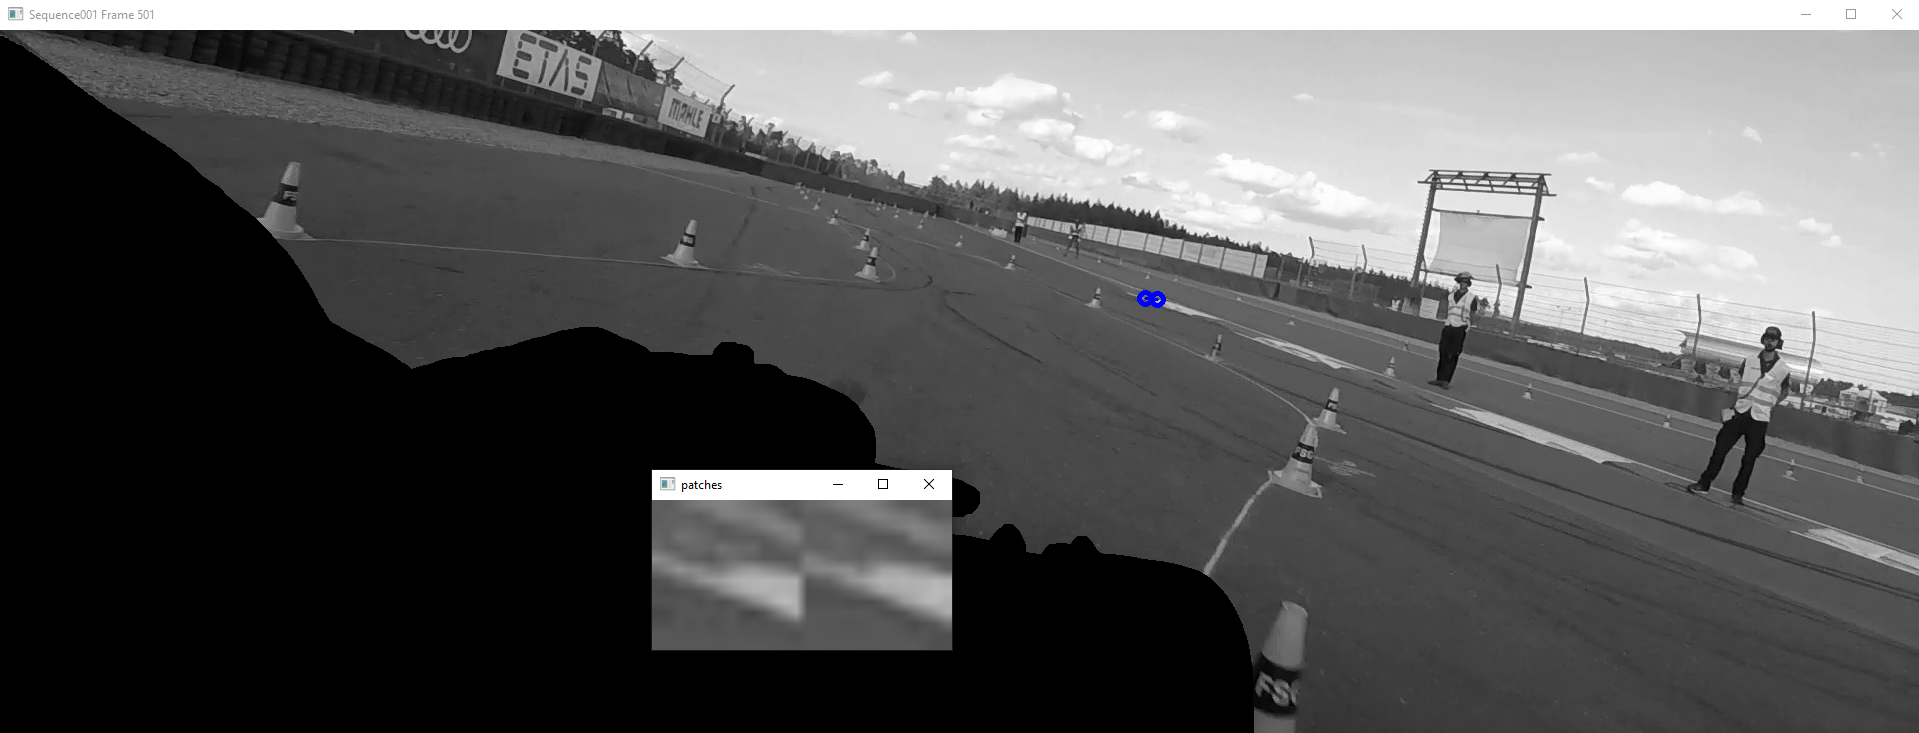
\includegraphics[width=\textwidth]{figures/match_checking.png}
    \caption{Confirming if this is a good match}
    \label{fig:match_check}
\end{figure}
\begin{figure}
    \centering
    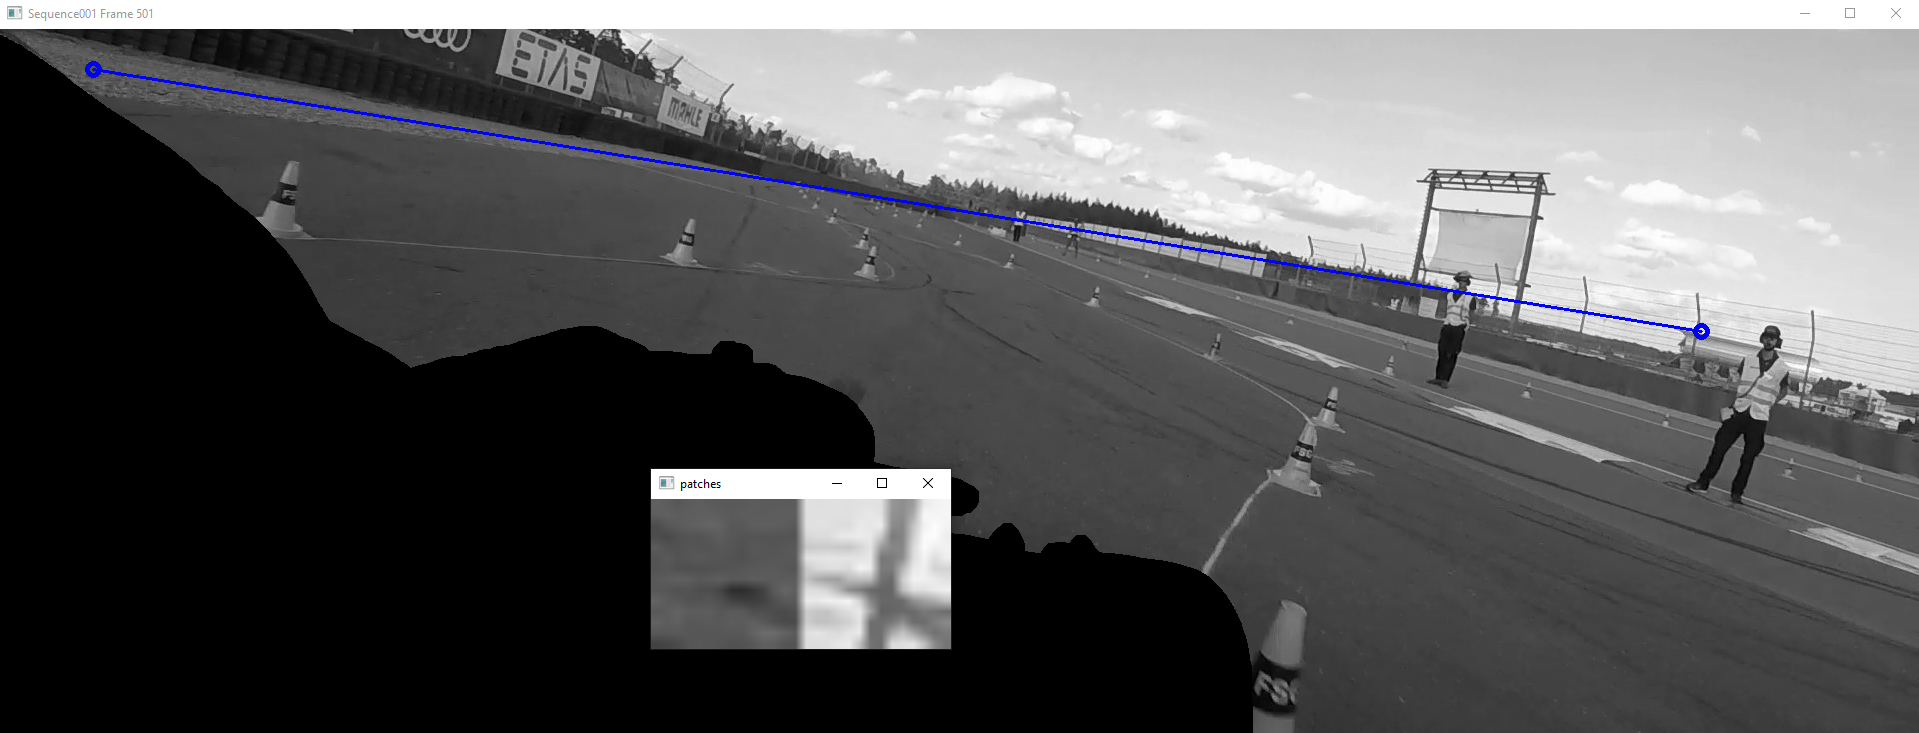
\includegraphics[width=\textwidth]{figures/match_checking_bad.png}
    \caption{Wrongly matched keypoints}
    \label{fig:bad_match}
\end{figure}

\section{Estimating 3D motion from sets of 2D point correspondences}
\subsection{Determining motion}
\subsubsection{Estimating homography}
We now have a good set of keypoint matches on the road surface. Using these, we can estimate the Homography between the road surfaces in the consecutive frames. Using the OpenCV method \textit{findHomography} we get a homography matrix. There are multiple methods in estimating the homography. When no parameter is given for the method, all keypoints are used to estimate the homography using the least squares method. Having one or multiple outliers has a big impact on this method and will return a faulty homography. \bigskip

\subsubsection{Random sample consensus (RANSAC)}
Using another method like RANSAC will make the estimation more robust to these outliers. RANSAC takes a random sample of the provided keypoints, calculates the homography based on this subset, then checks al keypoints for this homography and repeats this process to find the subset which works for the most keypoints. This subset is then called the consensus, all keypoints that are not a part of the consensus are considered outliers and will thus not be used to estimate the homography. 

\subsubsection{Decomposing the homography}
We now have a homography, using the OpenCV method \textit{decomposeHomograpyMat}, we get a list of possible rotation matrices, translation and normal vectors. To decompose the homography, we need to provide the intrinsic parameters of the camera we used, see \autoref{sec:cammodel}.